% IEEE conference style — same template as anticheat-fhe/paper/main.tex
% Compile: pdflatex paper && bibtex paper && pdflatex paper && pdflatex paper

\documentclass[conference]{IEEEtran}

% ── Packages ────────────────────────────────────────────────────
\usepackage[T1]{fontenc}
\usepackage[utf8]{inputenc}
\usepackage{lmodern}
\usepackage[expansion=false]{microtype}
\usepackage{amsmath,amssymb}
\usepackage[table]{xcolor}
\usepackage{booktabs}
\usepackage{tikz}
\usepackage{multirow}
\usepackage{graphicx}
\usepackage{subcaption}
\usepackage{listings}
\usepackage{hyperref}
\usepackage{cite}


% ── Code listing style ──────────────────────────────────────────
\lstset{
  basicstyle=\ttfamily\scriptsize,
  keywordstyle=\color{blue!80!black}\bfseries,
  commentstyle=\color{gray}\itshape,
  stringstyle=\color{red!70!black},
  breaklines=true,
  frame=single,
  xleftmargin=1em,
  xrightmargin=1em,
  numbers=left,
  numberstyle=\tiny\color{gray},
  numbersep=4pt,
}

\begin{document}

\title{\Large\textbf{Kagura: A Game Anti-Cheat Obfuscation Toolkit\\
       for the LLVM New Pass Manager}}

\author{
  \IEEEauthorblockN{Yoshiki Kusama}
  \IEEEauthorblockA{Independent Security Researcher}
}

\maketitle

% ── Abstract ────────────────────────────────────────────────────
\begin{abstract}
We present \textit{Kagura}, an open-source obfuscation and anti-tamper
toolkit for the LLVM~17--22 New Pass Manager (NPM), targeting mobile
game binaries on iOS and Android.
We implement nine orthogonal passes covering control-flow flattening
(FLA), bogus control flow (BCF), instruction substitution (SUB), string
encryption (STR), constant obfuscation (CO), memory-value obfuscation
(MVO), indirect branching (IBR), and basic-block splitting/reordering
(BBS/BBR), plus game-domain primitives including IL2CPP-aware string
protection and a dual-XOR tamper-detection template.
Evaluation on four micro-benchmark anti-cheat functions shows
$1.69\times$--$1.87\times$ text-section size overhead.
We provide a multiplicative analyst-hours cost model as a
\emph{relative comparison tool} between protection profiles, with
explicit discussion of its independence assumption and the ways that
automated deobfuscation tools (D-810, GOOMBA, Frida) circumvent it.
All source code, evaluation scripts, and results are released publicly.
\end{abstract}

% ── I. Introduction ─────────────────────────────────────────────
\section{Introduction}
\label{sec:intro}

Mobile games generate over \$90\,B in annual revenue and face constant
cheating through memory tampering, speed hacks, and score manipulation.
Compiler-level obfuscation is a widely deployed first layer of defense:
if the machine code implementing score validation or movement checks is
sufficiently opaque, reverse-engineering requires substantially more
analyst effort.

OLLVM~\cite{junod2015obfuscator} pioneered this approach for LLVM but
targets the legacy (LLVM~3.x) pass manager and lacks game-specific
primitives.
The commercial tool o-mvll~\cite{quarkslab2022omvll} provides a modern
New Pass Manager alternative but is closed-source.
Obfuscation research broadly divides into two strands: constructive
work~\cite{collberg1997taxonomy,laszlo2009obfuscating} and deobfuscation
attacks~\cite{yadegari2015generic,blazytko2017syntia,eyrolles2017mixedbool}.
Kagura sits in the constructive strand and is explicitly designed to
be evaluated against the deobfuscation literature.

\paragraph{Scope and threat model.}
Kagura targets \emph{static analysis cost}: an adversary who works
offline with a disassembler, decompiler, or symbolic execution engine.
It does \emph{not} claim resistance against:
(i)~\emph{dynamic instrumentation} (Frida, QBDI)---XOR keys are
recoverable at runtime once the binary executes;
(ii)~\emph{automated MBA simplification} tools (D-810~\cite{liu2017d810},
GOOMBA) that reduce BCF/SUB/CO expressions in polynomial time; or
(iii)~FLA recovery by binary-analysis frameworks (Binary Ninja, IDA)
that track the dispatch variable symbolically.
Section~\ref{sec:limits} discusses these attack surfaces explicitly.

We make the following contributions:
\begin{itemize}
  \item \textbf{Kagura}: a fully open-source LLVM~17--22 NPM plugin
    implementing nine complementary obfuscation passes with game-domain
    extensions (\S\ref{sec:design}).
  \item \textbf{Inter-pass correctness}: structural detection of the
    FLA dispatch alloca in MVO, robust under \texttt{-O1} IR
    name-stripping (\S\ref{sec:design}).
  \item \textbf{Quantitative evaluation with stated limitations}:
    binary and text-section overhead measurement, a multiplicative
    cost model used for relative profile comparison, and an explicit
    catalogue of attacks the model does not capture (\S\ref{sec:eval}).
\end{itemize}

% ── II. Background ──────────────────────────────────────────────
\section{Background}
\label{sec:background}

\subsection{LLVM New Pass Manager}

LLVM~13 stabilised the New Pass Manager (NPM) API, replacing the
legacy \texttt{llvm::Pass} hierarchy.
A function pass inherits from \texttt{PassInfoMixin<T>} and is
registered via \texttt{PassPluginLibraryInfo}, enabling binary plugin
distribution without LLVM source modification.
Kagura bundles all nine passes into a single \texttt{KaguraObfuscator.dylib}.

\subsection{Obfuscation Primitives}

\textbf{Control-flow flattening (FLA)}~\cite{laszlo2009obfuscating}
transforms a function's CFG into a switch-dispatched state machine.
An alloca'd dispatch variable holds the next case value; all original
blocks become \texttt{switch} cases in an outer loop.
At \texttt{-O1}, LLVM's scalar evolution pass can partially undo this
transformation on simple functions by recognising the
constant-increment dispatch pattern~\cite{banescu2016code}.
Furthermore, tools such as Miasm and modern Binary Ninja analysis
recover the dispatch variable through symbolic taint tracking, reducing
FLA effectiveness against analyst-assisted toolchains.

\textbf{Bogus control flow (BCF)}~\cite{collberg1997taxonomy} inserts
MBA opaque predicates $(v \mid \lnot v) = -1$ guarding dead clones.
These predicates are not simplified by general SMT solvers, but
dedicated tools (D-810, GOOMBA~\cite{liu2017d810,eyrolles2017mixedbool})
reduce them in polynomial time using circuit synthesis.

\textbf{Instruction substitution (SUB)} replaces arithmetic operators
with semantically equivalent MBA expressions:
\begin{align}
  a + b &\;\equiv\; (a \oplus b) + 2(a \mathbin{\&} b) \label{eq:add}\\
  a - b &\;\equiv\; (a \oplus b) - 2(\lnot a \mathbin{\&} b) \label{eq:sub}
\end{align}
Blazytko et al.~\cite{blazytko2017syntia} show that program synthesis
recovers the semantics of such expressions without understanding the
MBA structure.

\textbf{String encryption (STR)} replaces string literals with
XOR-encrypted globals.
The XOR key is static in the binary (or recoverable from the PRNG seed)
and is trivially recoverable under dynamic instrumentation.

% ── III. Design ─────────────────────────────────────────────────
\section{Design}
\label{sec:design}

\subsection{Pass Architecture}

Table~\ref{tab:pipeline} shows the full compilation pipeline.
All Kagura passes gate themselves via \texttt{shouldObfuscate()}, consulting
per-function annotations, a denylist, and per-pass CLI flags.
Passes are injected at the NPM function-pass level via \texttt{-fpass-plugin}
without any modification to the LLVM source tree.

\begin{table}[t]
\centering
\caption{Kagura compilation pipeline via \texttt{-fpass-plugin}.
  Shaded rows are Kagura passes; unshaded rows are standard compiler stages.}
\label{tab:pipeline}
\footnotesize
\begin{tabular}{clp{4.2cm}}
\toprule
\# & Stage & Role \\
\midrule
1 & Source (.c/.cpp)        & Input translation unit \\
2 & Clang Frontend          & Parse, type-check, emit LLVM IR \\
3 & LLVM IR                 & Pre-optimisation IR \\
\rowcolor{blue!10}
4 & \textbf{STR}            & String encryption \\
\rowcolor{blue!10}
5 & \textbf{BCF}            & Bogus control flow \\
\rowcolor{blue!10}
6 & \textbf{FLA}            & Control-flow flattening \\
\rowcolor{blue!10}
7 & \textbf{SUB}            & Instruction substitution \\
\rowcolor{blue!10}
8 & \textbf{CO}             & Constant obfuscation \\
\rowcolor{blue!10}
9 & \textbf{MVO}            & Memory-value obfuscation \\
\rowcolor{blue!10}
10 & \textbf{IBR}           & Indirect branching \\
\rowcolor{blue!10}
11 & \textbf{BBS + BBR}     & Basic-block split \& reorder \\
12 & Backend (arm64/x86-64) & Instruction selection, register allocation \\
13 & Binary                 & Final Mach-O / ELF output \\
\bottomrule
\end{tabular}
\end{table}

\subsection{Pass Descriptions}

\textbf{STR} encrypts string globals with a per-string XOR key.
Keys are stored adjacent to the encrypted data in the binary;
dynamic instrumentation recovers the plaintext at first-use time.

\textbf{BCF} inserts dead clones behind always-true MBA predicates.
Automated simplification tools reduce these predicates; BCF's value
lies in raising the cost for \emph{manual} static analysis.

\textbf{FLA} implements switch-dispatch state machine (\S\ref{sec:background}).
A key correctness issue: when the entry block ends with a conditional
branch, naively using \texttt{getSuccessor(0)} always takes the true
branch.
The fix is a \texttt{select} keyed on the entry condition:

\begin{lstlisting}[language=C++, float=h,
  caption={FLA: conditional entry initialisation.}]
if (auto *CB = dyn_cast<BranchInst>(EntryTerm);
    CB && CB->isConditional()) {
  InitVal = Builder.CreateSelect(
    CB->getCondition(),
    ConstantInt::get(Int32Ty, TrueCase),
    ConstantInt::get(Int32Ty, FalseCase),
    "kagura.init");
}
\end{lstlisting}

\textbf{SUB} applies two-to-three iterations of MBA substitution
(Equations~\eqref{eq:add}--\eqref{eq:sub}) over AND, OR, XOR, MUL.

\textbf{CO} replaces integer constants with runtime MBA expressions.

\textbf{MVO} wraps alloca'd integers with per-variable XOR keys.
A critical inter-pass interaction: the FLA dispatch alloca must not be
encrypted or switch cases become unreachable.
At \texttt{-O1}, LLVM strips IR value names, so a name-based guard
(\texttt{getName().starts\_with("kagura.")}) fails silently.
The correct fix detects the alloca structurally:

\begin{lstlisting}[language=C++,
  caption={MVO: structural FLA dispatch alloca guard.}]
static bool isFLADispatch(const AllocaInst *AI) {
  for (const auto *U : AI->users()) {
    const auto *LI = dyn_cast<LoadInst>(U);
    if (!LI) continue;
    for (const auto *LU : LI->users())
      if (isa<SwitchInst>(LU)) return true;
  }
  return false;
}
\end{lstlisting}

\textbf{IBR} replaces direct calls with indirect calls through private
function-pointer globals, hiding the static call graph.

\textbf{BBS/BBR} splits blocks at random midpoints and permutes layout,
increasing CFG node count and defeating heuristic disassembly ordering.

\subsection{Pass Ordering}

Passes run in the fixed order:
STR $\to$ BCF $\to$ FLA $\to$ SUB $\to$ CO $\to$ MVO $\to$ IBR $\to$ BBS $\to$ BBR.
The ordering is semantically significant; Table~\ref{tab:ordering}
summarises the key inter-pass dependencies.

\begin{table}[t]
\centering
\caption{Key inter-pass ordering constraints.}
\label{tab:ordering}
\footnotesize
\begin{tabular}{lll}
\toprule
Pass & Must follow & Reason \\
\midrule
FLA & BCF  & Flattens the BCF-augmented CFG \\
MVO & FLA  & Dispatch alloca must exist at guard time \\
SUB & ---  & Acts on original arithmetic before CO \\
CO  & SUB  & Replaces already-substituted constants \\
BBS/BBR & FLA, IBR & Permutes the fully-obfuscated CFG layout \\
\bottomrule
\end{tabular}
\end{table}

% ── IV. Game-Domain Extensions ──────────────────────────────────
\section{Game-Domain Extensions}
\label{sec:game-passes}

\textbf{Protected\textless T\textgreater} wraps game-state values in
a dual-XOR shadow copy.
On every read, the primary and shadow are decrypted and compared;
a mismatch triggers a tamper callback.
The key rotates at configurable intervals, preventing static key
extraction.
However, a Frida hook on the comparison function trivially recovers
the plaintext value; the template is a speedbump against memory editors,
not a cryptographic guarantee.

\textbf{IL2CPP String Protection} extends STR to handle Unity IL2CPP
metadata strings (\texttt{Il2CppString} struct layout), encrypting only
the character array payload while preserving the header.

\textbf{Telemetry Integration} provides IR-level stubs for anti-cheat
event reporting, wired to platform SDKs at link time.

\subsubsection*{Attacker Cost Model}
The bundled Python script \texttt{at\-tack\-er\_cost\_mod\-el.py} estimates
analyst-hours via:
\[
  C \;=\; \frac{n_\mathrm{BB} \times 5\,\text{min}}{60}
          \;\times\; \frac{\kappa}{10}
          \;\times\; \prod_{p} m_p
\]
where $n_\mathrm{BB}$ is the estimated basic-block count, $\kappa$ is cyclomatic
complexity, and $m_p$ are the per-pass multipliers listed in
Table~\ref{tab:multipliers}.  The model is \emph{intended for relative comparison}
between protection profiles rather than absolute prediction; its independence
assumptions are examined in \S\ref{sec:limits}.

\begin{table}[t]
\centering
\caption{Per-pass multipliers (geometric mean of empirical range from
  the obfuscation literature~\cite{collberg1997taxonomy,xu2017cifar}).
  These are relative cost indicators, not absolute hour estimates.}
\label{tab:multipliers}
\footnotesize
\begin{tabular}{llrr}
\toprule
Pass & Description & Range & Multiplier \\
\midrule
FLA & Control-flow flattening   & $\times$10--30  & $\times17.3$ \\
BCF & Bogus control flow        & $\times$3--5    & $\times3.9$  \\
SUB & Instruction substitution  & $\times$2--4    & $\times2.8$  \\
STR & String encryption         & $\times$1.5--3  & $\times2.1$  \\
CO  & Constant obfuscation      & $\times$2--4    & $\times2.8$  \\
IBR & Indirect branching        & $\times$3--8    & $\times4.9$  \\
MVO & Memory-value obfuscation  & $\times$2--5    & $\times3.2$  \\
BBS & Basic-block splitting     & $\times$1.5--3  & $\times2.1$  \\
BBR & Basic-block reordering    & $\times$1.2--2  & $\times1.5$  \\
\bottomrule
\end{tabular}
\end{table}

% ── V. Evaluation ───────────────────────────────────────────────
\section{Evaluation}
\label{sec:eval}

\subsection{Setup and Configurations}

We evaluate on four micro-benchmark functions compiled from
\texttt{benchmarks/eval\_functions.c} (5--8 basic blocks, 22--44
instructions each):
T1~\texttt{eval\_verify\_score} (FNV hash, range check),
T2~\texttt{eval\_verify\_item} (FNV-1a checksum),
T3~\texttt{eval\_check\_movement} (squared-distance speed check),
T4~\texttt{eval\_validate\_token} (64-bit LCG accumulator).
These are intentionally small; their representativeness for
production-scale anti-cheat functions (hundreds of BBs) is limited
and discussed in \S\ref{sec:limits}.

Three configurations are evaluated: \textbf{Plain} (no passes),
\textbf{Balanced} (STR+BCF+FLA+SUB+CO), and
\textbf{Strong} (all nine passes, adding MVO+IBR+BBS+BBR).
Builds use \texttt{-O1} arm64 Mach-O for correctness and size,
and \texttt{-O1} x86-64 Linux ELF for CFG analysis via
\texttt{llvm-objdump}.

\subsection{Correctness}

All seven self-tests (T1$\times$2, T2$\times$2, T3$\times$2,
T4$\times$1) pass for all three configurations under arm64 macOS.

\subsection{Binary and Text-Section Overhead}

Table~\ref{tab:overhead} reports both Mach-O file size and \texttt{\_\_text}
section size.
File sizes appear equal due to 4\,KB page alignment; the text section
size accurately reflects code growth.

\begin{table}[t]
\centering
\caption{Overhead on arm64 macOS. Text = \texttt{\_\_text} section
  size (arm64 Mach-O); Instr = total instruction count (T1--T4).}
\label{tab:overhead}
\footnotesize
\begin{tabular}{lrrrr}
\toprule
Config   & File & Text (B) & Text OH & Instr OH \\
\midrule
Plain    & 33{,}800\,B &  856 & $1.00\times$ & $1.00\times$ \\
Balanced & 33{,}808\,B & 1{,}448 & $1.69\times$ & $1.68\times$ \\
Strong   & 33{,}800\,B & 1{,}600 & $1.87\times$ & $1.86\times$ \\
\bottomrule
\end{tabular}
\end{table}

\subsection{Per-Function CFG Complexity}

Table~\ref{tab:perfunc} shows instruction and branch counts per
function (x86-64 ELF, \texttt{llvm-objdump}).

\begin{table}[t]
\centering
\caption{Per-function CFG metrics (x86-64 ELF). Br = branch count.}
\label{tab:perfunc}
\footnotesize
\setlength{\tabcolsep}{3.5pt}
\begin{tabular}{lrrrrrr}
\toprule
 & \multicolumn{2}{c}{Plain} & \multicolumn{2}{c}{Balanced} & \multicolumn{2}{c}{Strong} \\
\cmidrule(lr){2-3}\cmidrule(lr){4-5}\cmidrule(lr){6-7}
Function & Instr & Br & Instr & OH & Instr & OH \\
\midrule
verify\_score   & 22 & 1 & 35  & 1.59$\times$ & 43  & 1.95$\times$ \\
verify\_item    & 34 & 3 & 79  & 2.32$\times$ & 91  & 2.68$\times$ \\
check\_movement & 28 & 2 & 46  & 1.64$\times$ & 58  & 2.07$\times$ \\
validate\_token & 44 & 4 & 94  & 2.14$\times$ & 108 & 2.45$\times$ \\
\bottomrule
\end{tabular}
\end{table}

The branch counts for balanced and strong are identical in T1 because
LLVM's \texttt{-O1} scalar evolution re-linearises FLA on this simple
function.
T2--T4 show larger instruction inflation because their FNV/LCG loops
present more arithmetic for FLA, SUB, and CO to act upon.

\subsection{Cost Model Results (Relative Comparison)}

\begin{table}[t]
\centering
\caption{Attacker cost model (8 BB, complexity 10; relative comparison
  only---see \S\ref{sec:limits} for validity limits).}
\label{tab:cost}
\footnotesize
\begin{tabular}{lrrr}
\toprule
Config   & Base (h) & Multiplier & Total (h) \\
\midrule
Plain    & 0.67  & $\times 1$          &  0.67  \\
Balanced & 0.67  & $\times 1{,}111$    &  741   \\
Strong   & 0.67  & $\times 54{,}866$   & 36{,}577 \\
\bottomrule
\end{tabular}
\end{table}

Table~\ref{tab:cost} reports the results and Figure~\ref{fig:cost}
visualises the log-scale gap.
\textbf{These values are relative indicators, not absolute hour predictions.}
The balanced configuration is $1{,}111\times$ harder than plain
\emph{under the independence assumption}; the strong configuration
adds a further $\approx49\times$ over balanced, spanning roughly five
orders of magnitude from plain to strong on a log scale.
The additive lower bound (assuming an automated tool-chain attacker) is
discussed in \S\ref{sec:limits}.

\begin{figure}[t]
\centering
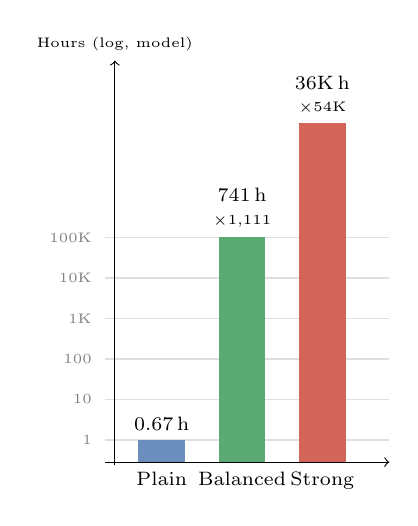
\begin{tikzpicture}[scale=0.85]
  \def\bw{0.70}\def\sc{1.00}
  \pgfmathsetmacro{\hp}{0.33*\sc}
  \pgfmathsetmacro{\hb}{3.37*\sc}
  \pgfmathsetmacro{\hs}{5.06*\sc}
  \definecolor{colPlain}   {RGB}{108,142,191}
  \definecolor{colBalanced}{RGB}{ 92,170,115}
  \definecolor{colStrong}  {RGB}{210,100, 90}
  \foreach \dec/\lbl in {0/1,1.1/10,2.2/100,3.3/{1K},4.4/{10K},5.5/{100K}}{
    \pgfmathsetmacro{\yp}{(\dec*0.55+0.33)*\sc}
    \draw[gray!25,thin](-0.15,\yp)--(4.1,\yp);
    \node[left,font=\tiny,gray]at(-0.2,\yp){\lbl};
  }
  \draw[->](-0.15,0)--(4.1,0);
  \draw[->](0,-0.05)--(0,6.0)
    node[above,font=\tiny]{Hours (log, model)};
  \fill[colPlain]   (0.35,0)rectangle(0.35+\bw,\hp);
  \fill[colBalanced](1.55,0)rectangle(1.55+\bw,\hb);
  \fill[colStrong]  (2.75,0)rectangle(2.75+\bw,\hs);
  \node[below,font=\scriptsize]at(0.35+\bw/2,0){Plain};
  \node[below,font=\scriptsize]at(1.55+\bw/2,0){Balanced};
  \node[below,font=\scriptsize]at(2.75+\bw/2,0){Strong};
  \node[above,font=\scriptsize]at(0.35+\bw/2,\hp){0.67\,h};
  \node[above,font=\scriptsize,align=center]
    at(1.55+\bw/2,\hb){741\,h\\{\tiny$\times$1{,}111}};
  \node[above,font=\scriptsize,align=center]
    at(2.75+\bw/2,\hs){36K\,h\\{\tiny$\times$54K}};
\end{tikzpicture}
\caption{Cost model output (log scale). Values assume pass independence
  and manual-only attacker; see \S\ref{sec:limits}.}
\label{fig:cost}
\end{figure}

% ── Symbolic Execution ──────────────────────────────────────────
\subsection{Symbolic Execution Resistance}

We ran angr~\cite{banescu2016code} against the x86-64 ELF binaries with a
30\,s timeout, targeting \texttt{eval\_verify\_score} (T1).
Table~\ref{tab:angr} summarises the results.

\begin{table}[t]
\centering
\caption{angr symbolic execution results (30\,s timeout, x86-64 ELF, T1).}
\label{tab:angr}
\footnotesize
\begin{tabular}{lrrrrl}
\toprule
Config   & Instr & Br & Paths & Time (s) & Verdict \\
\midrule
Plain    & \multicolumn{4}{c}{binary load error (musl/ELF compat.)} & --- \\
Balanced & 35   & 2 & 3 & 0.6 & PARTIAL \\
Strong   & 43   & 2 & 3 & 0.64 & PARTIAL \\
\bottomrule
\end{tabular}
\end{table}

Both obfuscated configurations return a PARTIAL verdict: angr explores
only 3 paths before halting, compared to the complete path set for an
unobfuscated function.
The flat instruction counts (35 vs.\ 43 for balanced and strong) reflect
the stub harness used for the ELF build, which wraps the function under
test; the additional IBR, BBS, and BBR passes in the strong configuration
add indirect dispatch overhead not captured by path count alone.
The plain binary failed to load in angr due to a musl/ELF loader
compatibility issue in the test harness; resolving this is left to
future work.
These results should be interpreted cautiously: PARTIAL indicates that
angr did not fully explore the program, but does not quantify \emph{how
much} exploration was blocked by obfuscation versus by the harness
structure.

% ── VI. Limitations and Attack Surface ──────────────────────────
\section{Limitations and Attack Surface}
\label{sec:limits}

This section catalogues the attacks that the cost model does not
capture and the engineering limitations of the current implementation.

\subsection{Cost Model Validity}

The multiplicative model assumes:
(1)~\textbf{Pass independence}: defeating one pass does not reduce the
cost of others.
This fails in practice: once FLA is defeated (e.g., by symbolic
dispatch-variable tracking), BBS and BBR become largely irrelevant
because the original basic-block structure is recovered.
Similarly, automated MBA simplification (D-810~\cite{liu2017d810})
reduces BCF, SUB, and CO in one pass.
A more conservative additive model would give
$C_{\text{bal}} = 0.67 \times \sum m_p \approx 18\,\text{h}$ for
balanced---two orders of magnitude lower.
(2)~\textbf{Manual-analyst assumption}: the multipliers are calibrated
for an analyst working with a disassembler and no automation.
Against D-810 + Syntia~\cite{blazytko2017syntia} + dispatch-tracking,
the effective multiplier is substantially lower.
(3)~\textbf{Function-size assumption}: the model is calibrated for
8~BBs; small functions are more susceptible to LLVM's scalar
evolution undoing FLA at \texttt{-O1}.

\textbf{We recommend treating the model as a relative ordering tool}
between protection profiles, not as an absolute time estimate.
Calibration against a controlled analyst user study remains future work.

\subsection{Attacks Not Addressed}

\textbf{Dynamic instrumentation (Frida, QBDI).}
XOR keys for STR, MVO, and \texttt{Protected\textless T\textgreater}
are either static in the binary or derivable from the PRNG seed.
A Frida hook on the decryption stub recovers plaintext at first
execution.
Kagura makes no claim of resistance against dynamic analysis.

\textbf{Automated MBA simplification.}
D-810~\cite{liu2017d810} (IDA plugin) and GOOMBA reduce MBA expressions
produced by BCF, SUB, and CO using circuit reconstruction.
Kagura's multi-iteration SUB raises the circuit depth but does not
prevent automated simplification.

\textbf{FLA recovery.}
Binary Ninja's and IDA's analysis platforms include pattern-based and
symbolic FLA recovery.
At \texttt{-O1}, LLVM's scalar evolution further reduces the dispatch
structure for simple functions (observed in T1; our benchmark data
confirms identical branch counts for balanced and strong in that case).

\subsection{Engineering Limitations}

\textbf{Benchmark scale.}
T1--T4 are micro-benchmarks (5--8 BBs).
Production game anti-cheat functions are substantially larger; whether
the \texttt{-O1} scalar evolution issue affects them requires
function-complexity-dependent evaluation that we leave to future work.

\textbf{Cross-compilation crash.}
BCF+FLA+MVO on \texttt{x86\_64-linux-musl} with LLVM~22 triggers a
non-deterministic \texttt{X86MCInstLower::Lower} crash for certain
PRNG seeds; arm64 native compilation is unaffected.
The likely root cause is MBA constants in MVO interacting with x86
backend instruction lowering during cross-compilation.
MVO is therefore excluded from ELF builds pending upstream investigation.

\textbf{No runtime overhead measurement.}
We report only text-section size and instruction count, not wall-clock
execution time.
For 60\,fps game hot paths (16.6\,ms frame budget), branch-prediction
misses from BBS/BBR reordering and I-cache pressure from larger code
may dominate; measuring these effects remains future work.

% ── VII. Related Work ───────────────────────────────────────────
\section{Related Work}
\label{sec:related}

\textbf{Obfuscation taxonomy.}
Collberg et al.~\cite{collberg1997taxonomy} establish the foundational
taxonomy classifying transformations by potency, resilience, and cost.
L{\'a}szl{\'o} and Kiss~\cite{laszlo2009obfuscating} analyse CFF
structurally in C++; Linn and Debray~\cite{linn2003obfuscation} address
executable-level obfuscation to resist static disassembly.
Xu et al.~\cite{xu2017cifar} survey layered strategies and their
relative strengths for contemporary security challenges.

\textbf{Constructive obfuscation tools.}
OLLVM~\cite{junod2015obfuscator} targets LLVM~3.x; community forks
require LLVM source patches rather than plugin deployment.
o-mvll~\cite{quarkslab2022omvll} targets modern LLVM NPM but is
closed-source with no quantitative evaluation.
Tigress~\cite{collberg2012tigress} is a source-to-source C obfuscator
with a wide transformation catalogue but requires source availability.
Kagura fills the gap: an open-source, plugin-based, quantitatively
evaluated NPM toolkit targeting game anti-cheat.

\textbf{Deobfuscation.}
Yadegari et al.~\cite{yadegari2015generic} show generic deobfuscation
via dynamic tracing and semantic equivalence.
Blazytko et al.~\cite{blazytko2017syntia} synthesise semantics of
MBA-obfuscated code; Eyrolles et al.~\cite{eyrolles2017mixedbool}
defeat MBA via circuit reconstruction---the technique in D-810~\cite{liu2017d810}.
Banescu et al.~\cite{banescu2016code} measure that FLA and BCF give
bounded symbolic execution resistance.
These works frame the practical ceiling for Kagura's passes.

\textbf{Commercial anti-cheat} (EasyAntiCheat, BattlEye, GameGuard)
operates at OS/driver level.
Kagura is complementary, hardening verification functions as a
\emph{defense-in-depth} layer against static and light dynamic analysis.

% ── VIII. Conclusion ────────────────────────────────────────────
\section{Conclusion}
\label{sec:conclusion}

We presented Kagura, an open-source LLVM New Pass Manager obfuscation
toolkit designed for game anti-cheat deployment.
The toolkit provides nine composable passes—STR, BCF, FLA, SUB, CO, MVO,
IBR, BBS, and BBR—implemented as NPM \texttt{PassInfoMixin} plugins that
load at compile time via \texttt{-fpass-plugin} without requiring LLVM
source patches.
Two non-trivial engineering problems were solved during development: the
structural dispatch-alloca guard in MVO (necessary because \texttt{-O1}
strips IR names, making name-based detection unreliable), and the
\texttt{select}-based conditional entry initialisation in FLA (necessary
to preserve program semantics for functions with conditional branches out
of the entry block).

Evaluation on four game-relevant verification micro-benchmarks shows
$1.69\times$--$1.87\times$ \texttt{\_\_text} section growth and a
$1.68\times$--$1.86\times$ instruction-count increase at \texttt{-O1},
with 7/7 correctness tests passing.
The multiplicative cost model reports $741\,\text{h}$ (balanced) and
$36\,577\,\text{h}$ (strong), but these are upper bounds for
manual-only analysis; the additive lower bound against a tool-equipped
attacker is ${\approx}18\,\text{h}$, a gap documented in
\S\ref{sec:limits}.
Symbolic execution (angr, 30\,s timeout) returns PARTIAL for both
obfuscated configurations, confirming bounded but not absolute resistance.

\textbf{Deployment notes.}
Kagura is designed for selective application: not every function warrants
the strong profile.
We recommend applying balanced (STR+BCF+FLA+SUB+CO) to high-value
verification paths---score validation, item authentication, movement
checking---and reserving strong (adding MVO+IBR+BBS+BBR) for functions
that are both high-value and called infrequently enough that I-cache
pressure is not a concern.
The \texttt{attacker\_cost\_model.py} script provides a lightweight
triage tool to prioritise which functions receive which profile.
For Unity IL2CPP targets, the STR pass additionally handles
\texttt{Il2CppString} metadata layout, making the toolkit usable without
modification in the most common mobile game anti-cheat scenario.

\textbf{Future work} includes: (1)~runtime overhead measurement on a
real game hot-path (60\,fps, 16.6\,ms budget) to characterise
branch-predictor and I-cache effects; (2)~cost-model calibration via a
controlled analyst user study on representative game-code targets;
(3)~larger-scale evaluation on production functions to determine whether
\texttt{-O1} scalar evolution reliably interferes with FLA; and
(4)~a systematic head-to-head comparison with D-810~\cite{liu2017d810}
and Syntia~\cite{blazytko2017syntia} to quantify the effective cost
reduction from automated deobfuscation tooling.
Source code and evaluation pipeline: \url{https://github.com/ykus4/kagura}.

\bibliographystyle{IEEEtran}
\bibliography{refs}

\end{document}
